\documentclass[11pt]{article}
\usepackage[utf8]{inputenc}
\usepackage[T1]{fontenc}
\usepackage[colorlinks=true, linkcolor=black]{hyperref}
\usepackage{amsthm}
\usepackage{enumitem}
\usepackage{amssymb}
\usepackage{amsmath}
\usepackage{amsfonts}
\usepackage[version=4]{mhchem}
\usepackage{stmaryrd}
\usepackage{mathrsfs}
\usepackage{graphicx}
\usepackage[export]{adjustbox}
\graphicspath{ {./images/} }

\title{\bf The theory of minimax approximation}


\author{Huaijin Wang}
\date{September 11, 2024}


\begin{document}

\maketitle
\newtheorem{definition}{Definition}[section]
\newtheorem{property}{Property}[section]
\newtheorem{lemma}{Lemma}[section]
\newtheorem{theorem}{Theorem}[]
\newtheorem{corollary}{Corollary}[section]
\newtheorem{remark}{Remark}[section]





\tableofcontents


\newpage
\section{Introduction to minimax approximation}

Let $\mathscr{C}[a, b]$ be the set of all continuous functions that are defined on the interval $[a,b]$ and $\mathscr{A}$ is a linear subspace of $\mathscr{C}[a,b]$ with finite dimensional.

The best minimax approximation from $\mathscr{A}$ to a function $f$ in $\mathscr{C}[a, b]$ is the element of $\mathscr{A}$ that minimizes the expression

\begin{equation}
\|f-p\|_{\infty}=\max _{a \leqslant x \leqslant b}|f(x)-p(x)|, \quad p \in \mathscr{A}. 
\label{eq:1}
\end{equation}
Thus, the best minimax approximation problem is given a function $f\in \mathscr{C}[a,b]$,
\begin{equation}
\left \{
\begin{aligned}
&\text{Find } p^* \in \mathscr{A} \text{ s.t.}\\
& \|f-p^*\|_\infty \leqslant \|f-p \|_\infty,\quad \forall p\in\mathscr{A}.
\end{aligned}
\right .
\label{problem:1}
\end{equation}

In this notes we study the conditions that are satisfied by a best approximation, when $\mathscr{A}$ is a general linear space.

We note that they take a particularly simple form if $\mathscr{A}$ is the space $\mathscr{P}_{n}$ of algebraic polynomials of degree at most $n$. 

In fact this form is obtained in the more general case when $\mathscr{A}$ satisfies the 'Haar condition', which is defined in Section 7.3. In Section 7.4 some further useful properties of best minimax approximations are proved in the case when the Haar condition is obtained, including the result that the best approximation is unique. 

The Haar condition also provides an excellent method for calculating best approximations, called the exchange algorithm, which is described in Chapter 8 and analysed in Chapter 9.\\

The theory that is developed for the case when $\mathscr{A}$ is any finite dimensional linear space comes from asking the following question. Let $p^{*}$ be a trial approximation from $\mathscr{A}$ to $f$. Can we find a change to $p^{*}$ that reduces the maximum error of the trial approximation? In other words, we seek an element $p$ in $\mathscr{A}$ such that the inequality


\begin{equation}
\left\|f-\left(p^{*}+\theta p\right)\right\|_{\infty}<\left\|f-p^{*}\right\|_{\infty} 
\label{ineq:1}
\end{equation}
is satisfied for some value of the scalar parameter $\theta$. Figure 7.1 gives an example to explain this point of view.

In the figure the function $f$, which is shown in each of the four parts, is to be approximated by a straight line, so $\mathscr{A}$ is the space $\mathscr{P}_{1}$. Three trial approximations, namely $p_{1}^{*}, p_{2}^{*}$ and $p_{3}^{*}$, are shown. The vertical lines in the figure indicate where the error function of each approximation takes its maximum value. We see that the straight line $p_{1}^{*}$ is not optimal, because the maximum error is reduced if the line is raised. The straight line $p_{2}^{*}$ is not optimal either, because the maximum error can be reduced


\begin{figure}[ht]
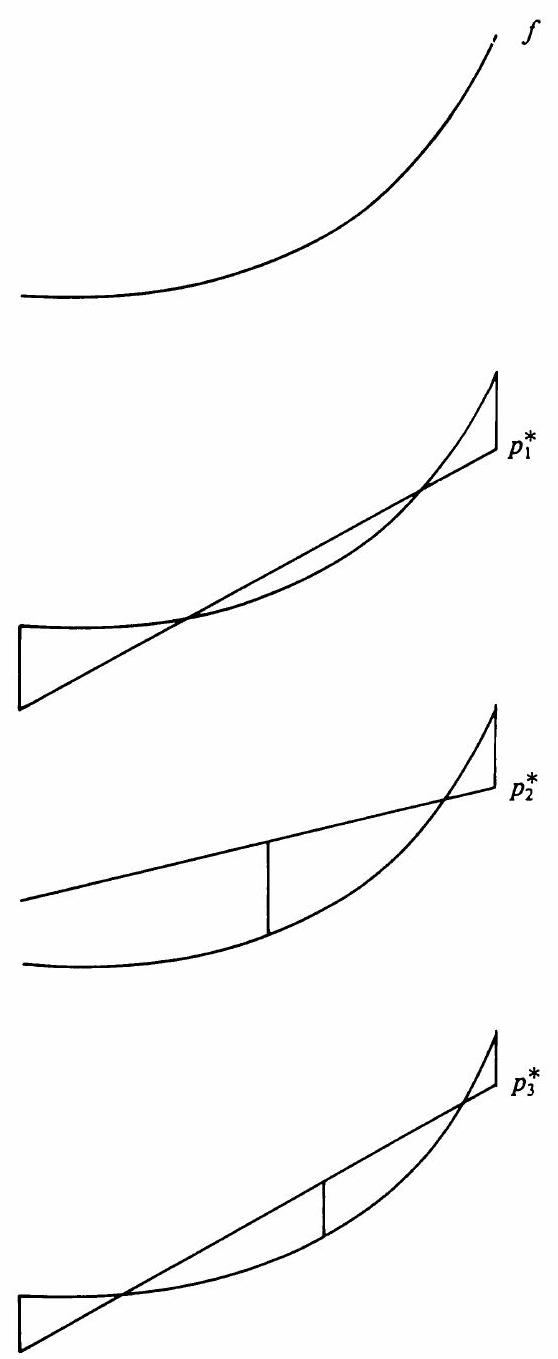
\includegraphics[max width=\textwidth, center]{2024_09_11_abbbcc72d07751cb658ag-084}
\caption{Figure 7.1. Minimax approximation by a straight line.}
\end{figure}
by rotating the line in a counter-clockwise direction. The straight line $p_{3}^{*}$, however, is the best approximation from $\mathscr{P}_{1}$ to $f$. We find in Section 7.3 that the characteristic property of a best straight line approximation is that the maximum error is achieved at three points of $[a, b]$ with alternating sign.

Figure 7.1 suggests that, to discover if a trial approximation is optimal, one only need consider the extreme values of the error function $\{f(x)-$ $\left.p^{*}(x) ; a \leqslant x \leqslant b\right\}$. This remark is made rigorous in the next section. It follows that we can find a function, $g$ say, to add to the function of Figure 7.1, such that the best approximation is unchanged, but the best approximation from $\mathscr{P}_{1}$ to $g$ is not the zero function. This remark is important, because it shows that in general a best minimax operator from $\mathscr{C}[a, b]$ to $\mathscr{A}$ is not a linear operator. Therefore the algorithms for calculating best approximations are iterative procedures.



\section{The reduction of the error of a trial approximation}

In this section, we consider the problem of how to deduce a "trial approximation" to a "better approximation".

Let $p^{*}$ be a trial approximation from $\mathscr{A}$ to a function $f$ in $\mathscr{C}[a, b]$, and we try to improve the approximation by satisfying condition \eqref{ineq:1}. The set of points at which the error function
\begin{equation}
e^{*}(x)=f(x)-p^{*}(x), \quad a \leqslant x \leqslant b, \label{eq:2}
\end{equation}
takes its extreme values is important, and we call it $\mathscr{Z}_{M}$, i.e., 
\begin{equation}
\mathscr{Z}_M = \{x\in [a,b]: \left|e^{*}(x)\right|=\left\|e^{*}\right\|_{\infty}\}.
\label{eq:3}
\end{equation}



We suppose first that $p^{*}$ is not optimal. We let $\left(p^{*}+\theta p\right)$ be a best approximation. Hence the reduction \eqref{ineq:1} is obtained, and the points in $\mathscr{Z}_{\mathrm{M}}$ satisfy the inequality


\begin{equation}
\left|e^{*}(x)-\theta p(x)\right|<\left|e^{*}(x)\right|, \quad x \in \mathscr{Z}_{\mathrm{M}} . \label{eq:4}
\end{equation}
We assume without loss of generality that $\theta$ is positive. Therefore expression (7.5) shows that, if $x$ is in $\mathscr{Z}_{\mathrm{M}}$, then the sign of $e^{*}(x)$ is the same as the sign of $p(x)$. In fact, this result is simplified as the conclusion: for any $a,b\in\mathbb{R}$, then $|a-b|<a$ implies that the sign of $a$ is the same as the sign of $b$.

\begin{lemma} \label{lem:1}
$p^{*}$ is a best minimax approximation from $\mathscr{A}$ to $f$ if there is no function $p$ in $\mathscr{A}$ that satisfies the condition
\begin{equation}
\left[f(x)-p^{*}(x)\right] p(x)>0, \quad x \in \mathscr{Z}_{\mathrm{M}} \label{ineq:2}
\end{equation}
\end{lemma}
\begin{proof}
If there is no function $p\in\mathscr{A}$ s.t. \eqref{ineq:2} holds, namely $\forall p\in\mathscr{A}$, we have 
\[
e^*(x) p(x) \leqslant 0,\quad \forall x\in\mathscr{Z}_M,
\]
where $e^*(x)$ is defined as in \eqref{eq:2}. Then
\[
\mathrm{sign}(e^*(x)) = -\mathrm{sign}(p(x)),\quad \forall x\in\mathscr{Z}_M.
\]
It leads to $\forall p\in \mathscr{A}$ and $\forall \theta>0$, 
\begin{equation}
\left | e^*(x) -\theta p(x)\right | \geqslant |e^*(x)|,\quad \forall x\in \mathscr{Z}_M.
\label{eq:5}
\end{equation}
Replace $(p^*-\theta p)$ with $p$ and take the maximum over $\mathscr{Z}_M$ on both sides of \eqref{eq:5}, leading to 
\[
\max_{x\in\mathscr{Z}_M } |f(x) - p^*(x)| \leqslant \max_{x\in\mathscr{Z}_M} |f(x) - p(x)|,\quad \forall p\in\mathscr{A}.
\]
Therefore, $\forall p\in\mathscr{A}$,
\[
\begin{aligned}
 \max_{a\leqslant x \leqslant b} |f(x) - p^*(x)| & = \max_{x\in\mathscr{Z}_M} |f(x) - p^*(x)| \\
& \leqslant \max_{x\in\mathscr{Z}_M} |f(x) - p(x)| \leqslant \max_{a\leqslant x\leqslant b} |f(x) - p(x)|.
\end{aligned}
\]
\end{proof}


In the remainder of this section the converse result of Lemma \ref{lem:1} is proved, namely that, if inequality \eqref{ineq:2} holds for some $p$ in $\mathscr{A}$, then there exists a positive value of $\theta$ that gives the reduction \eqref{ineq:1}.

Because of the way in which the exchange algorithm works, we generalize the problem of minimizing $\|f-p\|_{\infty}$, to be a more general case.

Let $\mathscr{Z}$ be any closed subset of $[a,b]$, which may be $[a,b]$ itself, or just composed of a finite number of points. Then, we consider the problem: for given $f\in\mathscr{C}[a,b]$,
\begin{equation}
\left \{
\begin{aligned}
&\text{Find } p^*\in\mathscr{A} \text{ s.t.}\\
& \max_{x\in\mathscr{Z}} |f(x) - p^*(x)| \leqslant \max_{x\in \mathscr{Z}} |f(x) - p(x)|,\quad \forall p\in \mathscr{A}.
\end{aligned}
\right .
\label{problem:2}
\end{equation}

\begin{remark}
Compared with the problem of \eqref{problem:1}, the problem of \eqref{problem:2} would be more general and focus on the the local property which will be more suitable for computation.
\end{remark}


\begin{theorem} \label{thm:1}
Let $\mathscr{A}$ be a linear subspace of $\mathscr{C}[a, b]$, let $f$ be any function in $\mathscr{C}[a, b]$, let $\mathscr{Z}$ be any closed subset of $[a, b]$, let $p^{*}$ be any element of $\mathscr{A}$, and let $\mathscr{Z}_{\mathrm{M}}$ be the set of points of $\mathscr{Z}$ at which the error $\left\{\left|f(x)-p^{*}(x)\right| ; x \in\right.$ $\mathscr{Z}\}$ takes its maximum value, i.e.,
\[
\mathscr{Z}_M = \{x^*\in\mathscr{Z}: |f(x^*) - p^*(x^*)| = \max_{x\in\mathscr{Z}} |f(x)-p^*(x)| \}.
\]
Then $p^{*}\in\mathscr{A}$ is a minimax approximation that satisfies \eqref{problem:2} if and only if there is no function $p$ in $\mathscr{A}$ that satisfies condition \eqref{ineq:2}.
\end{theorem}

\begin{proof}
{\bf Sufficiency.} The proof is really the same as it does in Lemma \ref{lem:1}. Suppose that there is no function $p\in\mathscr{A}$ that satisfies \eqref{ineq:2}, then $\forall p\in\mathscr{A}$ there holds
\[
[f(x) - p^*(x)] p(x) \leqslant 0,\quad \forall x\in \mathscr{Z}_M.
\]
Namely, the sign of $p(x)$ is different to the sign of $e^*(x)$ as $x$ ranges over $\mathscr{Z}_M$, i.e.,
\[
\mathrm{sign}(e^*(x)) = -\mathrm{sign}(p(x)),\quad \forall x\in\mathscr{Z}_M.
\]
It leads to $\forall p\in\mathscr{A}$ and $\forall \theta>0$,
\[
|e^*(x) - \theta p(x)| \geqslant |e^*(x)|,\quad \forall x\in \mathscr{Z}_M.
\]
Then, $\forall p\in\mathscr{A}$,
\[
\max_{x\in\mathscr{Z}_M} |f(x) - p(x)| \geqslant \max_{x\in\mathscr{Z}_M} |f(x) - p^*(x)|.
\]
Hence $\forall p\in \mathscr{A}$,
\[
\begin{aligned}
\max_{x\in\mathscr{Z}} |f(x) - p^*(x)| & = \max_{x\in \mathscr{Z}_m} |f(x) - p^*(x)| \\ 
& \leqslant \max_{x\in\mathscr{Z}_M} |f(x) - p(x)| \leqslant \max_{x\in\mathscr{Z}} |f(x) - p(x)|.
\end{aligned}
\]

 {\bf Necessity.} We prove it by contraction. Suppose that $p\in \mathscr{A}$ that satisfies \eqref{ineq:2}. We need to show that there exists $\theta>0$ such that 
 \begin{equation}
 \max_{x\in\mathscr{Z}} |e^*(x) - \theta p(x)| < \max_{x\in \mathscr{Z}} |e^*(x)|.
 \label{ineq:3}
 \end{equation}
 
 Without loss of generality, we assume 
 \[
 |p(x)| \leqslant 1,\quad \forall x\in [a,b].
 \]
 Let
 \[
 \mathscr{Z}_0 := \{x_0\in\mathscr{Z}: p(x_0) e^*(x_0) \leqslant 0 \}.
 \]
 It is obvious that $\mathscr{Z}_0$ is closed, and because $\mathscr{Z}_0$ and $\mathscr{Z}_M$ have no common points, the number
\[
d = \max_{x\in\mathscr{Z}_0} |e^*(x)|
\]
satisfies the bound
\[
d < \max_{x\in \mathscr{Z}} |e^*(x)|.
\]
If $\mathscr{Z}_0=\varnothing$, we denote $d=0$. 
(Note that the inequality strictly holds since $|e^*(x)|$ achieves its maximum on $\mathscr{Z}_M$, but not $\mathscr{Z}_0$, and $\mathscr{Z}_0 \cap \mathscr{Z}_M = \varnothing$). 

We will show that \eqref{ineq:3} holds with $\theta$ as
\[
\theta = \frac{1}{2} \left [\max_{x\in\mathscr{Z}} |e^*(x)| - d \right ].
\]

Because $\mathscr{Z}$ is closed, there must be a $\xi \in \mathscr{Z}$ such that 
\[
|e^*(\xi) - \theta p(\xi)| = \max_{x\in\mathscr{Z}} |e^*(x)-\theta p(x)|.
\]
\begin{itemize}
\item If $\xi\in\mathscr{Z}_0$, the bound
\[
\begin{aligned}
\max_{x\in\mathscr{Z}} |e^*(x) - \theta p(x)| & = |e^*(\xi)| + |\theta p(\xi)| \leqslant d + \theta \\
& = \frac{1}{2} \left[ \max_{x\in\mathscr{Z}} |e^*(x)| + \max_{x\in\mathscr{Z}_0} |e^*(x)|\right ] \\
& < \max_{x\in\mathscr{Z}} |e^*(x)|,
\end{aligned}
\]
where the first equal holds because the sign of $e^*(x)$ is the same as the sign of $p(x)$ as we assume that $p(x)$ satisfies \eqref{ineq:2}.

\item If $\xi \notin \mathscr{Z}_0$, then $\mathrm{sign}(e^*(\xi)) = \mathrm{sign}(p(\xi))$ and
\[
|e^*(\xi) - \theta p(\xi)| < \max \left[ |e^*(x)|, |\theta p(\xi)|\right].
\]
By the facts that 
\[
\begin{aligned}
& |e^*(\xi)|   \leqslant \max_{x\in\mathscr{Z}} |e^*(x)|, \\
& |\theta p(\xi) |  \leqslant \theta = \frac{1}{2} \left[ \max_{x\in\mathscr{Z}} |e^*(x)| - \max_{x\in\mathscr{Z}_0} |e^*(x)|\right ] \leqslant \max_{x\in\mathscr{Z}} |e^*(x)|.
\end{aligned}
\]
It follows that \eqref{ineq:3} is satisfied.
\end{itemize}
\end{proof}

Theorem \ref{thm:1} suggests that to find out if a trial approximation is optimal, one only need consider the extreme values of the error function. Specifically, one should ask if condition \eqref{ineq:2} holds for some function $p$ in $\mathscr{A}$.

\section{The characterization theorem and the Haar condition} \label{sec:3}
If the set $\mathscr{A}$ of approximating functions is the space $\mathscr{P}_{n}$ of algebraic polynomials of degree at most $n$, then it is rather easy to test whether condition \eqref{ineq:2} can be obtained. We make use of the fact that a function in $\mathscr{P}_{n}$ has at most $n$ sign changes. Therefore, if the error function $\left[f(x)-p^{*}(x)\right]$ changes sign more than $n$ times as $x$ ranges over $\mathscr{Z}_{\mathrm{M}}$, then $p^{*}$ is a best approximation. Conversely, if the number of sign changes does not exceed $n$, then we can choose the zeros of a polynomial in $\mathscr{P}_{n}$ so that condition \eqref{ineq:2} is satisfied. This result is usually called the minimax characterization theorem, and it is stated formally below.

It is useful to express the theorem in a form that applies to a class of functions that includes polynomials as a special case. The usual way of defining this class is to identify the properties of polynomials that are used in the proof of the characterization theorem. They are the following two conditions:
\begin{enumerate}[label=(\arabic*)]
\item If an element of $\mathscr{P}_{n}$ has more than $n$ zeros, then it is identically zero.

\item Let $\left\{\zeta_{i} ; j=1,2, \ldots, k\right\}$ be any set of distinct points in the open interval ( $a, b$ ), where $k \leqslant n$. There exists an element of $\mathscr{P}_{n}$ that changes sign at these points, and that has no other zeros. Moreover, there is a function in $\mathscr{P}_{n}$ that has no zeros in $[a, b]$.

\hspace{-2em} The following two properties of polynomials are required later:

\item If a function in $\mathscr{P}_{n}$, that is not identically zero, has $j$ zeros, and if $k$ of these zeros are interior points of $[a, b]$ at which the function does not change sign, then the number $(j+k)$ is not greater than $n$.

\item Let $\left\{\xi_{j} ; j=0,1, \ldots, n\right\}$ be any set of distinct points in $[a, b]$, and let $\left\{\phi_{i} ; i=0,1, \ldots, n\right\}$ be any basis of $\mathscr{P}_{n}$. Then the $(n+1) \times$ $(n+1)$ matrix whose elements have the values $\left\{\phi_{i}\left(\xi_{j}\right)\right.$; $i=0,1, \ldots, n ; j=0,1, \ldots, n\}$ is non-singular.
\end{enumerate}

\begin{remark}
Condition (2) states that there exists two kind of polynomials in $\mathscr{P}_n$ such that only $k$ roots at which sign changes contained in $(a,b)$, or no zeros in $[a,b]$.
\end{remark}

An $(n+1)$-dimensional linear subspace $\mathscr{A}$ of $\mathscr{C}[a, b]$ is said to satisfy the {\it 'Haar condition'} if these four statements remain true when $\mathscr{P}_{n}$ is replaced by the set $\mathscr{A}$. Let's rewrite the definition just to be a little bit more specific:

\begin{definition}[Haar Condition]The $(n+1)$-dimensional linear subspace $\mathscr{A}$ of $\mathscr{C}[a, b]$ is said to satisfy the Haar condition if these four statements remain true 

\begin{enumerate}[label=(\arabic*)]
\item If an element of $\mathscr{A}$ has more than $n$ zeros, then it is identically zero.

\item Let $\left\{\zeta_{i} ; j=1,2, \ldots, k\right\}$ be any set of distinct points in the open interval ( $a, b$ ), where $k \leqslant n$. There exists an element of $\mathscr{A}$ that changes sign at these points, and that has no other zeros. Moreover, there is a function in $\mathscr{A}$ that has no zeros in $[a, b]$.

\item If a function in $\mathscr{A}$, that is not identically zero, has $j$ zeros, and if $k$ of these zeros are interior points of $[a, b]$ at which the function does not change sign, then the number $(j+k)$ is not greater than $n$.

\item Let $\left\{\xi_{j} ; j=0,1, \ldots, n\right\}$ be any set of distinct points in $[a, b]$, and let $\left\{\phi_{i} ; i=0,1, \ldots, n\right\}$ be any basis of $\mathscr{A}$. Then the $(n+1) \times$ $(n+1)$ matrix whose elements have the values $\left\{\phi_{i}\left(\xi_{j}\right)\right.$; $i=0,1, \ldots, n ; j=0,1, \ldots, n\}$ is non-singular.
\end{enumerate}
\end{definition}

\begin{remark}
Equivalently, any basis of $\mathscr{A}$ is called a 'Chebyshev set'. Spaces that satisfy the Haar condition are studied in Appendix A. It is proved that properties (1), (3) and (4) are equivalent, and that these properties imply condition (2). It is usual to define the Haar condition in terms of the first property. Thus $\mathscr{A}$ satisfies the Haar condition if and only if, for every non-zero $p$ in $\mathscr{A}$, the number of roots of the equation $\{p(x)=0 : a \leqslant x \leqslant b\}$ is less than the dimension of $\mathscr{A}$.
\end{remark}

\begin{remark}
It is also useful to define the Haar condition in terms of the Chebyshev system: 
$\mathscr{A}$ satisfies the Haar condition if and only if any basis with $(n+1)$ elements of $\mathscr{A}$ constitutes a Chebyshev system.
\end{remark}



\begin{theorem}[Characterization Theorem] \label{thm:2}
Let $\mathscr{A}$ be an $(n+1)$-dimensional linear subspace of $\mathscr{C}[a, b]$ that satisfies the Haar condition, and let $f$ be any function in $\mathscr{C}[a, b]$. Then $p^{*}$ is the best minimax approximation from $\mathscr{A}$ to $f$, if and only if there exist $(n+2)$ points $\left\{\xi_{i}^{*}: i=0,1, \ldots, n+1\right\}$, such that the conditions
\begin{align}
& a \leqslant \xi_{0}^{*}<\xi_{1}^{*}<\ldots<\xi_{n+1}^{*} \leqslant b, \label{eq:6} \\
& \left|f\left(\xi_{i}^{*}\right)-p^{*}\left(\xi_{i}^{*}\right)\right|=\left\|f-p^{*}\right\|_{\infty}, \quad i=0,1, \ldots, n+1 \label{eq:7}
\end{align}
and
\begin{equation}
f\left(\xi_{i+1}^{*}\right)-p^{*}\left(\xi_{i+1}^{*}\right)=-\left[f\left(\xi_{i}^{*}\right)-p^{*}\left(\xi_{i}^{*}\right)\right], \quad i=0,1, \ldots, n \label{eq:8}
\end{equation}
are obtained.
\end{theorem}

\begin{proof}
{\bf Necessity.} Suppose that $p^*$ is the best minimax approximation from $\mathscr{A}$ to $f$. Let $\mathscr{Z}_M$ be the set for which $|f(x)-p^*(x)|$ attains its maximum, i.e.,
$$
\mathscr{Z}_M = \{x^* \in [a,b]: |f(x^*) - p^*(x^*)| = \max_{a\leqslant x \leqslant b} |f(x) - p^*(x)| \}.
$$
We claim that the number of elements in $\mathscr{Z}_M$, denoted as $n(\mathscr{Z}_M)$, is at least $n+2$. Otherwise, if $n(\mathscr{Z}_M) \leqslant n+1$, we can show that there exists a function $p\in\mathscr{A}$ s.t.
$$
[f(x)-p^*(x)] p(x) >0,\quad \forall x\in\mathscr{Z}_M,
$$
which contradicts our assumption by the conclusion in Theorem \ref{thm:1}.

In fact, we can
suppose that $\mathscr{Z}_M = \{\xi_1,\xi_2,\cdots,\xi_{m}\}$, where $m \leqslant n+1$ and $\xi_i\neq\xi_j$ for $i\neq j$. Let $\{\phi_i(x)\}_{i=1}^{n+1}$ be a basis of $\mathscr{A}$, and we assume that $p$ could be expanded as the form
$$
p(x) = \sum_{j=1}^{n+1} \alpha_j \phi_j(x),\quad \text{for some } \alpha_j, \ j=1,2,\cdots,n+1.
$$
Let $p$ satisfy $p(\xi_i) = \mathrm{sign}[f(\xi_i)-p^*(\xi_i)]$, which leads to
$$
p(\xi_i) = \sum_{j=1}^{n+1} \alpha_j \phi_j(\xi_i) = \mathrm{sign}[f(\xi_i)-p^*(\xi_i)], \quad i=1,2,\cdots,m.
$$
The linear system has non-zero solutions for $\alpha_j$. Thus such a $p(x)$ does exist.

We claim again that $f(x)-p^*(x)$ changes sign at least $n+1$ times as $x$ ranges over $\mathscr{Z}_M$. Otherwise, if $f(x)-p^*(x)$ changes sign at most $n$ times, we suppose that its value at $\zeta_1,\zeta_2,\cdots,\zeta_{n+1} \in \mathscr{Z}_M$ has different signs, i.e., 
$$
f(\zeta_i) - p^*(\zeta_i) = (-1)^i \lambda \|f-p^*\|_\infty,\quad i=1,2,\cdots,n+1,
$$
where $\lambda = 1\text{ or } -1$. Then we can find $p\in\mathscr{A}$ such that 
$$
[f(\zeta_i) - p^*(\zeta_i)] p(\zeta_i) > 0,\quad i=1,\cdots,n+1,
$$
since any basis of $\mathscr{A}$ constitutes a Chebyshev set.

Hence we have shown that $f(x)-p^*(x)$ changes sign at least $n+1$ times as $x$ ranges over $\mathscr{Z}_M$, which is the sufficient condition of this theorem.

{\bf Sufficiency.} Suppose that conditions \eqref{eq:6}, \eqref{eq:7} and \eqref{eq:8} are satisfied, and then $p^*\in\mathscr{A}$ such that $f(x) - p^*(x)$ cahnges sign at least $n+1$ times as $x$ ranges over $\mathscr{Z}_M$. We claim that there is no function $p\in\mathscr{A}$ such that 
$$
[f(\xi_i^*) - p^*(\xi^*_i)] p(\xi_i^*) > 0, \quad i=0,1,\cdots,n+1.
$$
Otherwise, if such $p$ does exist, then the sign of $p(\xi^*_i)$ is as same as the sign of $f(\xi^*_i)-p^*(\xi^*_i)$, i.e.,
$$
\mathrm{sign}(p(\xi^*_i)) = \mathrm{sign}[f(\xi^*_i)-p^*(\xi^*_i)],\quad i=0,1,\cdots,n+1.
$$
By the condition \eqref{eq:8}, we have 
$$
\mathrm{sign}(p(\xi^*_{i+1})) = - \mathrm{sign}(p(\xi^*_i)),\quad i=0,1,\cdots,n.
$$
Then $p(x)$ has at least $n+1$ zeros. By Haar conditions, we obtain $p\equiv 0$, which leads to a contradiction. Hence this claim is proved which implies $p^*$ is the best minimax approximation by virtue of Theorem \ref{thm:1}.
\end{proof}

\begin{remark}
One important application of this theorem is to prove the minimum property of Chebyshev polynomials.
\end{remark}

 We recall that the Chebyshev polynomial $T_{n}$ is the polynomial of degree $n$ that is defined on the interval $[-1,1]$ by the equation


\begin{equation}
T_{n}(x)=\cos (n \theta), \quad x=\cos \theta, \quad 0 \leqslant \theta \leqslant \pi \label{eq:9}
\end{equation}


The minimum property is sufficiently useful to be stated as a theorem.

\begin{theorem} \label{thm:3}
Let the range of $x$ be $[-1,1]$, and let $n$ be any positive integer. The polynomial $\left(\frac{1}{2}\right)^{n-1} T_{n}$ is the member of $\mathscr{P}_{n}$, whose $\infty$-norm is least, subject to the condition that the coefficient of $x^{n}$ is equal to one.
\end{theorem}
\begin{proof}
One way of identifying the required polynomial is to solve the problem
$$
\left \{
    \begin{aligned}
        &\text{Find } \{c^*_i: i=0,1,\cdots,n-1\} \text{ s.t.} \\
        &\max_{-1\leqslant x \leqslant 1} \left |x^n + \sum_{i=0}^{n-1} c^*_i x^i \right | \leqslant 
        \max_{-1\leqslant x \leqslant 1} \left |x^n + \sum_{i=0}^{n-1} c_i x^i \right |,\quad \forall c_i.
    \end{aligned}
\right .
$$
We see that this approach is equivalent to finding the best minimax approximation from $\mathbb{P}_{n-1}$ to the function $x^n$ in the interval $[-1,1]$.

It follows from Theorem \ref{thm:2} that $(\frac{1}{2})^{n-1} T_n$ is the required polynomial, if the coefficient of $x^n$ is one, and if there exist points $\{\xi_i: i=0,1\cdots,n\}$ in $[-1,1]$ arranged in ascending order, such that the equations
\begin{equation}
T_n(\xi_i) = (-1)^{n-i} \|T_n\|_\infty,\quad i=0,1,\cdots,n, \label{eq:10}
\end{equation}
hold. The recurrence relation of Tchebyshev polynomials implies that the coefficient of $x^n$ is correct. Moreover, the definition \eqref{eq:9} shows that equation \eqref{eq:10} is satisfied if we let each $\xi_i$ have the value $\cos[(n-i)\pi/n]$. The theorem is proved.
\end{proof}

\begin{remark}
The main reason for letting $\mathscr{Z}$ be any closed subset of $\mathscr{C}[a, b]$ in the statement of Theorem 7.1, is that the exchange algorithm requires the case when $\mathscr{Z}$ contains just $(n+2)$ points. In descriptions of the exchange algorithm it is usual to call such a set of points a 'reference'. We use this term also, and we let $\left\{\xi_{i} ; i=0,1, \ldots, n+1\right\}$ be the points of the reference. We assume that always these points are in ascending order
\begin{equation*}
a \leqslant \xi_{0}<\xi_{1}<\ldots<\xi_{n+1} \leqslant b \tag{7.23}
\end{equation*}
\end{remark}



The following corollary of Theorem 7.1 is used on every iteration of the exchange algorithm.

\begin{theorem} \label{thm:4}
Let $\mathscr{A}$ be an $(n+1)$-dimensional linear subspace of $\mathscr{C}[a, b]$ that satisfies the Haar condition, let $\left\{\xi_{i} ; i=0,1, \ldots, n+1\right\}$ be a reference, and let $f$ be any function in $\mathscr{C}[a, b]$. Then $p^{*}$ is the function in $\mathscr{A}$ that minimizes the expression
\begin{equation}
\max _{i=0,1, \ldots, n+1}\left|f\left(\xi_{i}\right)-p\left(\xi_{i}\right)\right|, \quad p \in \mathscr{A} \label{eq:11}
\end{equation}
if and only if the equations
\begin{equation}
f\left(\xi_{i+1}\right)-p^{*}\left(\xi_{i+1}\right)=-\left[f\left(\xi_{i}\right)-p^{*}\left(\xi_{i}\right)\right], \quad i=0,1, \ldots, n \label{eq:12}
\end{equation}
are satisfied.
\end{theorem}

\begin{proof}
Let $\mathscr{Z} = \{\xi_0,\xi_1,\cdots,\xi_{n+1} \}$, and $\mathscr{Z}_M \subset \mathscr{Z}$ be the set for which $|f(x)-p^*(x)|$ attains its maximum, i.e.,
$$
\mathscr{Z}_M = \{x^*\in \mathscr{Z}: |f(x^*) - p^*(x^*)| = \max_{0\leqslant i\leqslant n+1} |f(\xi_i) - p^*(\xi_i)| \}.
$$
By Theorem \ref{thm:1}, $p^*$ is the best minimax approximation over the set $\mathscr{Z}$, i.e.,
$$
\max_{0\leqslant i\leqslant n+1} |f(\xi_i) - p^*(\xi_i) | \leqslant \max_{0\leqslant i \leqslant n+1} |f(\xi_i) - p(\xi_i)|,\quad \forall p\in\mathscr{A},
$$
if and only if there is no function $p\in \mathscr{A}$ such that 
$$
[f(x) - p^*(x)] p(x) >0,\quad \forall x\in\mathscr{Z}_M.
$$

{\bf Necessity.} We claim that $\mathscr{Z}_M = \mathscr{Z}$. In fact, if it is not true, then the number of elements in $\mathscr{Z}_M$ is at most $n+1$, and then we can show there exists a function $p\in\mathscr{A}$ such that
$$
[f(x) - p^*(x)] p(x) >0,\quad \forall x\in\mathscr{Z}_M,
$$
which leads to a contradiction. (See the proof of Theorem \ref{thm:2}).
Then we proved that $\mathscr{Z}_M = \mathscr{Z}$. Hence, we can show that $f(x)-p^*(x)$ changes sign at least $n+1$ times as $x$ ranges over $\mathscr{Z}_M$. (See the proof of Theorem \ref{thm:2})

{\bf Sufficiency.} We assume that \eqref{eq:12} holds. Then it is obvious that $\mathscr{Z}_M=\mathscr{Z}$. We can show a proof by contradiction that there is no function $p\in\mathscr{A}$ such that 
$$
[f(x) - p^*(x)] p(x) >0,\quad \forall x\in\mathscr{Z}_M,
$$
holds.
\end{proof}


The function $p^{*}$ that minimizes expression \eqref{eq:11} may be calculated from the equations \eqref{eq:12}. It is usual to let $h$ be the value of $\left[f\left(\xi_{0}\right)-\right.$ $\left.p^{*}\left(\xi_{0}\right)\right]$, and to choose a basis of $\mathscr{A},\left\{\phi_{j} ; j=0,1, \ldots, n\right\}$ say. It follows that the coefficients of the function
\begin{equation*}
p^{*}(x)=\sum_{j=0}^{n} \lambda_{j} \phi_{j}(x), \quad a \leqslant x \leqslant b \tag{7.26}
\end{equation*}
satisfy the equations
\begin{equation*}
f\left(\xi_{i}\right)-\sum_{j=0}^{n} \lambda_{j} \phi_{j}\left(\xi_{i}\right)=(-1)^{i} h, \quad i=0,1, \ldots, n+1 \tag{7.27}
\end{equation*}
which is a linear system in the unknowns $\left\{\lambda_{j} ; j=0,1, \ldots, n\right\}$ and $h$. Because Theorem \ref{thm:4} shows that these equations have a solution for all functions $f$ in $\mathscr{C}[a, b]$, the matrix of the system is non-singular. Hence only one element of $\mathscr{A}$ minimizes expression \eqref{eq:11}. A more general and more useful method of proving uniqueness is given in the next section.

\section{Uniqueness and bounds on the minimax error}
Suppose that the conditions of Theorem \ref{thm:2} hold, that $p^{*}$ and $q^{*}$ are both best minimax approximations from $\mathscr{A}$ to $f$, and that conditions \eqref{eq:6}, \eqref{eq:7} and \eqref{eq:8} are satisfied. We let $r^{*}$ be the function $\left(q^{*}-p^{*}\right)$, and we consider the numbers
\begin{equation}
r^{*}\left(\xi_{i}^{*}\right)=\left[f\left(\xi_{i}^{*}\right)-p^{*}\left(\xi_{i}^{*}\right)\right]-\left[f\left(\xi_{i}^{*}\right)-q^{*}\left(\xi_{i}^{*}\right)\right],\quad 
i  =0,1, \ldots, n+1 \label{eq:18}
\end{equation}


Because $\left\|f-q^{*}\right\|_{\infty}$ and $\left\|f-p^{*}\right\|_{\infty}$ are equal, it follows from equation \eqref{eq:7}
that either $r^{*}\left(\xi_{i}^{*}\right)$ is zero, or its sign is the same as the sign of $\left[f\left(\xi_{i}^{*}\right)-\right.$ $\left.p^{*}\left(\xi_{i}^{*}\right)\right]$. Hence equation \eqref{eq:8} provides information about the signs of the terms of the sequence $\left\{r^{*}\left(\xi_{i}^{*}\right) ; i=0,1, \ldots, n+1\right\}$. 

It can be deduced from this information that $r^{*}$ is identically zero. (Since $r^*\in\mathscr{A}$ and it has at least $n+1$ zeros, by Haar condition, which leads to it identically zero).

 Hence the best minimax approximation from $\mathscr{A}$ to $f$ is unique. The method of proving that $r^{*}$ is identically zero is a general one that has several applications. Therefore it is stated in the following theorem.

\begin{theorem} \label{thm:5}
Let $r$ be a function in $\mathscr{C}[a, b]$, and let $\left\{\xi_{i} : i=0,1, \ldots, n+1\right\}$ be a reference, such that the conditions
\begin{equation}
(-1)^{i} r\left(\xi_{i}\right) \geqslant 0, \quad i=0,1, \ldots, n+1 \label{eq:13}
\end{equation}
are satisfied. Then $r$ has at least $(n+1)$ zeros in $[a, b]$, provided that any double zero is counted twice, where a double zero is a zero that is strictly inside $[a, b]$, at which $r$ does not change sign.
\end{theorem}

\begin{proof}
Let $\mathscr{I}$ and $\mathscr{J}$ be the sets
\begin{equation}
\left.\begin{array}{ll}
\mathscr{I}=\left\{i: r\left(\xi_{i}\right) \neq 0,\right. & i=0,1, \ldots, n+1\}  \\
\mathscr{J}=\left\{j: r\left(\xi_{i}\right)=0,\right. & j=0,1, \ldots, n+1\}
\end{array}\right\},
\label{eq:14}
\end{equation}

and let $n(\mathscr{I})$ and $n(\mathscr{F})$ be the number of elements in each set. The theorem is trivial if $n(\mathscr{F})$ is zero or one. Otherwise we consider the number of zeros in the interval $\left[\xi_{k}, \xi_{l}\right]$, where $k$ and $l$ are both in $\mathscr{I}$, and where no other element of $\mathscr{I}$ is in the range $[k, l]$. Condition \eqref{eq:13} implies that the numbers $r\left(\xi_{k}\right)$ and $r\left(\xi_{l}\right)$ have the same sign if $(l-k)$ is even, and they have opposite signs if $(l-k)$ is odd. Hence the number of zeros of $r$ in the interval $\left[\xi_{k}, \xi_{l}\right]$ is at least one more than the number of points of the set $\left\{\xi_{j} ; j \in \mathscr{J}\right\}$ that are in this interval, provided that any double zero is counted twice. Because the number of pairs $\left[\xi_{k}, \xi_{l}\right]$ that have this property is $[n(\mathscr{I})-1]$, it follows that the total number of zeros of $r$ in $[a, b]$ is at least $[n(\mathscr{I})+n(\mathscr{J})-1]$, which is the required result. $\quad \square$
\end{proof}

Hence we obtain the uniqueness theorem for best approximation in the $\infty$-norm.

\begin{theorem} \label{thm:6}
Let $\mathscr{A}$ be a linear subspace of $\mathscr{C}[a, b]$ that satisfies the Haar condition. Then, for any $f$ in $\mathscr{C}[a, b]$, there is just one best minimax approximation from $\mathscr{A}$ to $f$.
\end{theorem}
\begin{proof}
Suppose that $p^{*}$ and $q^{*}$ are both best approximations. Let $r^*(x) = \left(p^{*}(x)-q^{*}(x) \right)$. Then by Theorem \ref{thm:2}, there exist $(n+2)$ points $\{\xi_i^*: i = 0,1,\cdots,n+1\}$ such that \eqref{eq:6}, \eqref{eq:7} and \eqref{eq:8} are satisfied. Then for $i=0,1,\cdots,n+1$,
\[
| f(\xi_i^*) - q^*(\xi_i^*) | \leqslant \|f-q^*\|_\infty = \|f-p^*\|_\infty = |f(\xi_i^*) - p^*(\xi_i^*)|.
\]
By expression \eqref{eq:18}, $r^*(\xi_i^*)$ is either zero or
\[
\mathrm{sign}(r^*(\xi_i^*)) = \mathrm{sign}(f(\xi_i^*) - p^*(\xi_i^*)).
\]
Therefore, 
\[
\mathrm{sign}(r^*(\xi_{i+1}^*)) = -\mathrm{sign}(r^*(\xi_i^*)),\quad i=0,1,\cdots,n,
\]
where we define $\mathrm{sign}(0)=1$. Then 
\[
(-1)^i \lambda r^*(\xi_i^*) \geqslant 0,\quad i=0,1,\cdots,n+1,
\]
for which $\lambda=1$ or $-1$ is a constant. By Theorem \ref{thm:5}, $r^*(x)$ has at least $n+1$ zeros in $[a,b]$ and $r^*(x)\in\mathscr{A}$. It follows from property (1) of Haar condition, that $r^*(x)$ is identically zero.
\end{proof}

\begin{remark}
Another interesting property of the Haar condition, which is the subject of Exercise 7.9, is that, if $\mathscr{A}$ is any finite-dimensional linear subspace of $\mathscr{C}[a, b]$ that does not satisfy the Haar condition, then there are functions $f$ in $\mathscr{C}[a, b]$ that have several best approximations in $\mathscr{A}$.
\end{remark}

Theorem \ref{thm:5} is also useful for obtaining lower bounds on the least value of expression \eqref{eq:1}. Suppose that an iterative method for calculating a best approximation produces a trial approximation $p^{*}$, and that the conditions \eqref{eq:6}, \eqref{eq:7} and \eqref{eq:8} are almost satisfied. Then we usually have available a reference $\left\{\xi_{i} : i=0,1, \ldots, n+1\right\}$, such that the signs of the terms 
$$\left\{f\left(\xi_{i}\right)-p^{*}\left(\xi_{i}\right) : i=0,1, \ldots, n+1\right\}
$$
alternate. In this case the following theorem applies.

\begin{theorem} \label{thm:7}
Let the conditions of Theorem \ref{thm:2} hold, let $p^{*}$ be any element of $\mathscr{A}$, and let $\left\{\xi_{i} ; i=0,1, \ldots, n+1\right\}$ be a reference, such that the condition
\begin{equation}
\operatorname{sign}\left[f\left(\xi_{i+1}\right)-p^{*}\left(\xi_{i+1}\right)\right]=-\operatorname{sign}\left[f\left(\xi_{i}\right)-p^{*}\left(\xi_{i}\right)\right],\quad 
i  =0,1, \ldots, n \label{eq:15}
\end{equation}
is satisfied. Then the inequalities
\begin{equation}
\begin{aligned}
\min _{i=0,1, \ldots, n+1}\left|f\left(\xi_{i}\right)-p^{*}\left(\xi_{i}\right)\right| & \leqslant \min _{p \in \mathscr{A}} \max _{i=0,1, \ldots, n+1}\left|f\left(\xi_{i}\right)-p\left(\xi_{i}\right)\right| \\
& \leqslant \min _{p \in \mathscr{A}}\|f-p\|_{\infty} \\
& \leqslant\left\|f-p^{*}\right\|_{\infty} 
\end{aligned}\label{eq:16}
\end{equation}
are obtained. Moreover, the first inequality is strict unless all the numbers $\left\{\left|f\left(\xi_{i}\right)-p^{*}\left(\xi_{i}\right)\right| : i=0,1, \ldots, n+1\right\}$ are equal.
\end{theorem}

\begin{proof}
The third inequality of expression \eqref{eq:16} holds because $p^{*}$ is in $\mathscr{A}$, and the second one holds because the reference is a subset of $[a, b]$. In the next we prove the first inequality, i.e.,
\begin{equation}
\min_{0\leqslant i \leqslant n+1} |f(\xi_i) - p^*(\xi_i)| \leqslant 
\min_{p\in\mathscr{A}} \max_{0\leqslant i \leqslant n+1} |f(\xi_i) - p(\xi_i)|.
\label{eq:20}
\end{equation}
By contradiction, we suppose that \eqref{eq:20} is not hold, i.e.,
\[
\min_{0\leqslant i \leqslant n+1} |f(\xi_i) - p^*(\xi_i)| >
\min_{p\in\mathscr{A}} \max_{0\leqslant i \leqslant n+1} |f(\xi_i) - p(\xi_i)|.
\]
Since $\mathscr{A}$ is finite dimensional and then it is a closed subspace. There exists $q^*(x) \in \mathscr{A}$ such that
\[
\min_{0\leqslant i \leqslant n+1} |f(\xi_i) - p^*(\xi_i)| >
\max_{0\leqslant i \leqslant n+1} |f(\xi_i) - q^*(\xi_i)|.
\]
Then we have 
\[
|f(\xi_i) - p^*(\xi_i)| > |f(\xi_i) - q^*(\xi_i)|,\quad i=0,1,\cdots,n+1.
\]
We set $r^* = q^* - p^*$ as defined in \eqref{eq:18}, then it is obvious that 
$\mathrm{sign} (r^*(\xi_i) ) = \mathrm{sign} (f(\xi_i) - p^*(\xi_i))$ and by \eqref{eq:15},  that $r^*$ has at least $n+1$ zeros in $[a,b]$. It follows that $r^*\equiv 0$ from $r^*\in\mathscr{A}$ and condition (1) of Haar condition. Therefore $q^* = p^*$, which leads to
\[
\min_{0\leqslant i \leqslant n+1} |f(\xi_i) - p^*(\xi_i)| > \max_{0\leqslant i\leqslant n+1} |f(\xi_i) - p^*(\xi_i)|,
\]
which is a contradiction.

Finally, we prove the proposition: the equal sign of \eqref{eq:20} holds if and only if all the numbers $\left\{\left|f\left(\xi_{i}\right)-p^{*}\left(\xi_{i}\right)\right|: i=0,1, \ldots, n+1\right\}$ are equal.

{\bf Necessity}

We suppose that 
\[
\min_{0\leqslant i \leqslant n+1} |f(\xi_i) - p^*(\xi_i)| =
\min_{p\in\mathscr{A}} \max_{0\leqslant i \leqslant n+1} |f(\xi_i) - p(\xi_i)|.
\]
Then there exists $q^*\in\mathscr{A}$ such that
\[
\min_{0\leqslant i \leqslant n+1} |f(\xi_i) - p^*(\xi_i)| =
\max_{0\leqslant i \leqslant n+1} |f(\xi_i) - q^*(\xi_i)|.
\]
We can prove that $q^* = p^*$ by contradiction.
Then 
\[
\min_{0\leqslant i \leqslant n+1} |f(\xi_i) - p^*(\xi_i)| = \max_{0\leqslant i \leqslant n+1} |f(\xi_i) - p^*(\xi_i)|,
\]
which leads to $|f(\xi_i) - p^*(\xi_i)|$ are the same.

{\bf Sufficiency}

By Theorem \ref{thm:4}.

\end{proof}

It is useful to note that, if $p^{*}$ is the best minimax approximation from $\mathscr{A}$ to $f$, and if the reference in the statement of the last theorem is the set of points $\left\{\xi_{i}^{*} ; i=0,1, \ldots, n+1\right\}$ that occurs in conditions \eqref{eq:6}, \eqref{eq:7} and \eqref{eq:8}, then all the inequalities of expression \eqref{eq:16} are satisfied as equations.

\section{Appendix}
Notation Interpretation:
\begin{itemize}
\item $\mathscr{A}$ Linear space of $\mathscr{C}[a,b]$
\end{itemize}

\end{document}